\chapter{Discussion of the Results}
\label{chap:results-analysis}

This chapter analyzes the results reported in Chapter~\ref{chap:probing-results} for each of the eight models and both datasets. Section~\ref{sec:ch8-gpt-oss} analyzes the results of GPT-OSS 20B separately, due to its difference from the other models stated in Chapter~\ref{chap:probing-results}, and because, among all the models, it is the only one where the results in Chapter~\ref{chap:probing-results} show a probe that is less accurate than the coordinator. The following sections then analyze the other seven models together.

Section~\ref{sec:ch8-overview} compares the probe against the coordinator, on the whole dataset, across the difficulty tiers and across the two interaction settings, and answers \hyperref[rq:ch8-rq1-intro]{\textbf{RQ1}}. Section~\ref{sec:ch8-failure-analysis} compares the failures of the probe, of the coordinator and of the text-only classifiers, and answers \hyperref[rq:ch8-rq2-intro]{\textbf{RQ2}}. Section~\ref{sec:ch8-depth} reports the relative depth of the optimal layer for the probe, and answers \hyperref[rq:ch8-rq3-intro]{\textbf{RQ3}}. Section~\ref{sec:ch8-error-flag} evaluates the probe as a runtime error flag on the coordinator's decision, and answers \hyperref[rq:ch8-rq4-intro]{\textbf{RQ4}}.

% many floats: let pages end short instead of stretching the text to the bottom
\raggedbottom

\section{Probe Underperformance on GPT-OSS 20B}
\label{sec:ch8-gpt-oss}

Among the eight models of Section~\ref{sec:ch7-results}, GPT-OSS 20B is the only one whose chain-of-thought output cannot be disabled (Section~\ref{subsec:ch7-reasoning-traces}). In its runs, a reasoning output is generated after the prompt and before the tool call that states the routing decision. GPT-OSS 20B is also the only model where the probe is less accurate than the coordinator. This section analyzes its two runs in detail, to determine whether the hidden state at the last prompt token may be insufficient to predict the choice of the sub-agent when the reasoning output cannot be disabled.

\begin{table}[htbp]
    \centering
    \begin{tabular}{@{}lcccc@{}}
        \toprule
        \textbf{Dataset} & \textbf{\begin{tabular}[b]{@{}c@{}}probe\\AUC macro\end{tabular}} & \textbf{\begin{tabular}[b]{@{}c@{}}probe AUC macro,\\other seven models\end{tabular}} & \textbf{\begin{tabular}[b]{@{}c@{}}coordinator\\accuracy\end{tabular}} & \textbf{\begin{tabular}[b]{@{}c@{}}probe\\accuracy\end{tabular}} \\
        \midrule
        Single-turn & 0.915 & 0.974--0.989 & \textbf{0.818} & 0.689 \\
        Multi-turn  & 0.788 & 0.928--0.979 & \textbf{0.719} & 0.505 \\
        \bottomrule
    \end{tabular}
    \caption[\texttt{gpt-oss-20b} probe AUC macro and coordinator accuracy]{\texttt{gpt-oss-20b}: AUC macro of the probe at its optimal layer, range of the same metric across the other seven models, accuracy of the coordinator and accuracy of the probe, from Section~\ref{sec:ch7-results}.}
    \label{tab:ch8-gpt-oss-exception}
\end{table}

Table~\ref{tab:ch8-gpt-oss-exception} shows that the accuracy of the probe is lower than the accuracy of the coordinator by 0.129 on the single-turn dataset and by 0.214 on the multi-turn dataset. On both datasets, the AUC macro of the probe is also below the range of the other seven models. The sub-agents are therefore less separable in the hidden states of GPT-OSS 20B than in those of any other model analyzed in this work.

\subsection{Probing at the Last Reasoning Token}
\label{subsec:ch8-gpt-oss-reasoning}

The probe reads the hidden state at the last prompt token, before the reasoning output is generated. For the other seven models the tool call follows the prompt directly, but for GPT-OSS 20B the choice of the sub-agent may be formed during the reasoning process. The representation at the last prompt token may therefore be insufficient to train a linear probe that can separate the sub-agents accurately.

To test this reading, a second simulation of GPT-OSS 20B was run on the single-turn dataset to capture the hidden states at the last token of the reasoning output. A probe was then trained on these hidden states at every layer, with the same procedure used at the last prompt token (Section~\ref{sec:ch7-probing-setup}). Table~\ref{tab:ch8-gpt-oss-reasoning} compares the probe at the last prompt token, reported in Section~\ref{subsec:ch7-gpt-oss-20b}, with the probe at the last reasoning token. Figure~\ref{fig:ch8-gpt-oss-reasoning-routers} compares the probe at the last reasoning token with the coordinator's decision and the text-only baselines, and its layer sweep is reported in Appendix~\ref{chap:appendix-layer-sweeps}.

\begin{table}[htbp]
    \centering
    \small
    \setlength{\tabcolsep}{3.5pt}
    \begin{tabular}{@{}lcccccccccc@{}}
        \toprule
        & & & \multicolumn{4}{c}{\textbf{all}} & \multicolumn{4}{c}{\textbf{adversarial}} \\
        \cmidrule(lr){4-7} \cmidrule(lr){8-11}
        & \textbf{optimal layer} & \textbf{AUC macro} & \textbf{model} & \textbf{probe} & $\boldsymbol{\Delta}$ & $\boldsymbol{p_{\text{holm}}}$ & \textbf{model} & \textbf{probe} & $\boldsymbol{\Delta}$ & $\boldsymbol{p_{\text{holm}}}$ \\
        \midrule
        Prompt & 18/24 & 0.915 & 0.818 & 0.689 & \rgain{-0.129} & $<10^{-4}$ & 0.737 & 0.601 & \rgain{-0.136} & $<10^{-4}$ \\
        Reasoning & 16/24 & 0.936 & 0.818 & 0.796 & \rgain{-0.022} & 0.026 & 0.737 & 0.719 & \rgain{-0.018} & \pns{0.20} \\
        \bottomrule
    \end{tabular}
    \caption[\texttt{gpt-oss-20b}, probe against model at the last prompt and reasoning token]{\texttt{gpt-oss-20b}, single-turn, probe against model at the last prompt token (Prompt) and at the last reasoning token (Reasoning). A $p_{\text{holm}}$ followed by (n.s.) is not significant at the 0.05 threshold.}
    \label{tab:ch8-gpt-oss-reasoning}
\end{table}

\begin{figure}[htbp]
    \centering
    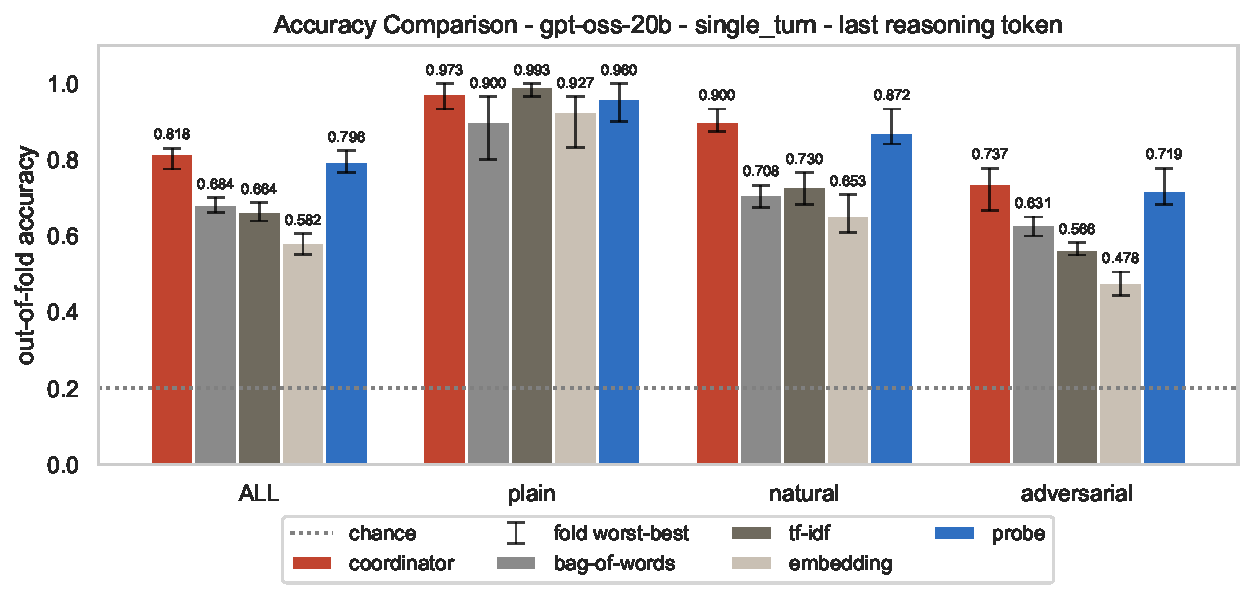
\includegraphics[width=0.85\textwidth]{images/models/gpt-oss-20b_single_turn_reasoning_routers.pdf}
    \caption[Accuracy comparison, gpt-oss-20b, single-turn, probe at the last reasoning token]{Accuracy comparison, gpt-oss-20b, single-turn, probe at the last reasoning token.}
    \label{fig:ch8-gpt-oss-reasoning-routers}
\end{figure}

\subsection{Observations}
\label{subsec:ch8-gpt-oss-observations}

At the last reasoning token, the AUC macro of the probe rises from 0.915 to 0.936. The accuracy of the probe rises from 0.689 to 0.796 on the whole dataset and from 0.601 to 0.719 on the \texttt{adversarial} tier. The probe exceeds all three text-only baselines on the whole dataset and on the \texttt{natural} and \texttt{adversarial} tiers, and its accuracy gets close to the accuracy of the coordinator without exceeding it. The accuracy of the coordinator exceeds the accuracy of the probe by 0.022 on the whole dataset and 0.018 on the \texttt{adversarial} tier. According to the McNemar test, the difference is significant on the whole dataset ($p_{\text{holm}} = 0.026$) but not on the \texttt{adversarial} tier ($p_{\text{holm}} = 0.20$).

A possible reason is that, before the last reasoning token, the model has already generated a reasoning output that discusses the sub-agents and reaches a conclusion. The hidden state during reasoning summarizes the input and the reasoning generated so far, and it is updated as the reasoning proceeds towards a final answer \cite{luStreamingHallucinationDetection2026}. The hidden state at the last reasoning token may therefore be skewed towards the sub-agent the model chose. This does not happen for the other seven models, where the probe reads the hidden state before any output is generated. This reading is consistent with the fraction of samples where the probe predicts the same sub-agent as the coordinator, which rises from 0.672 at the last prompt token to 0.866 at the last reasoning token. A probe trained from this state may therefore mostly learn the decision of the coordinator, including its errors, which would explain why its accuracy approaches the accuracy of the coordinator without exceeding it.

For GPT-OSS 20B, the hidden state at the last prompt token may not yet encode enough information to predict the choice of the sub-agent, because that choice depends on the reasoning generated afterward. The hidden state at the last reasoning token, in contrast, may already reflect that choice, since the reasoning that leads to it has already been generated.

\subsection{Effect on the Rest of the Analysis}
\label{subsec:ch8-gpt-oss-exclusion}

Both probe positions examined in this section have a limitation for GPT-OSS 20B. At the last prompt token, the hidden state may not yet encode the choice of the sub-agent, because that choice may be formed during the reasoning output. At the last reasoning token, the hidden state may already reflect that choice, so the probe may mostly learn the decision of the coordinator, including its errors.

The results of GPT-OSS 20B are therefore excluded from Sections~\ref{sec:ch8-overview} to~\ref{sec:ch8-error-flag}, so that they are not pooled with the results of the other seven models.

\FloatBarrier


\section{Comparison of Coordinator and Probe Accuracy}
\label{sec:ch8-overview}

\phantomsection\label{rq:ch8-rq1-intro}
\begin{rqbox}[RQ1]
On requests where the correct sub-agent is difficult to determine from the wording alone, does a probe on the hidden states of a coordinator model recover the correct sub-agent more accurately than the coordinator's own selection?
\end{rqbox}


\noindent To answer \hyperref[rq:ch8-rq1-intro]{\textbf{RQ1}}, this section compares the accuracy of the probe with the accuracy of the coordinator on both datasets and on each difficulty tier. The comparison across the difficulty tiers shows how the accuracy of the probe changes against the accuracy of the coordinator as the difficulty increases. The comparison between the two datasets shows how the multi-turn setting affects the accuracy.

The correct sub-agent is difficult to determine from the wording alone when text-only classifiers reach a low accuracy on the request (Section~\ref{subsec:lexical-separability}). The difficulty tiers lower this accuracy from \texttt{plain} to \texttt{adversarial} (Section~\ref{sec:dataset-baselines}).

\subsection{Accuracy on the Whole Dataset}
\label{subsec:ch8-overview-all}

Table~\ref{tab:ch8-overview} reports, from Section~\ref{sec:ch7-results}, the AUC macro of the probe, the accuracy of the coordinator and of the probe, their difference, and the McNemar test between the two, Holm-corrected as in Chapter~\ref{chap:probing-results}. The \emph{margin} $\Delta$ is the difference between the two accuracies, computed as the accuracy of the probe minus the accuracy of the coordinator.

\begin{table}[htbp]
    \centering
    \small
    \setlength{\tabcolsep}{4pt}
        \begin{tabular}{@{}lccccc@{}}
            \toprule
            \textbf{Model} & \textbf{\begin{tabular}[b]{@{}c@{}}probe\\AUC macro\end{tabular}} & \textbf{\begin{tabular}[b]{@{}c@{}}coordinator\\accuracy\end{tabular}} & \textbf{\begin{tabular}[b]{@{}c@{}}probe\\accuracy\end{tabular}} & $\boldsymbol{\Delta}$ & $\boldsymbol{p_{\text{holm}}}$ \\
            \midrule
            \multicolumn{6}{@{}l}{\textit{Single-turn}} \\
            \midrule
            \texttt{gemma4-e2b-it} & 0.976 & \worst{0.736} & 0.848 & \rgain{0.112} & $<10^{-4}$ \\
            \texttt{qwen3-4b} & 0.977 & 0.752 & 0.864 & \rgain{0.112} & $<10^{-4}$ \\
            \texttt{qwen3-8b} & 0.974 & 0.772 & \worst{0.845} & \rgain{0.073} & $<10^{-4}$ \\
            \texttt{gemma4-12b-it} & 0.988 & 0.873 & 0.916 & \rgain{0.043} & $<10^{-4}$ \\
            \texttt{gemma4-26b-a4b-it} & 0.989 & \best{0.888} & \best{0.921} & \rgain{0.033} & 0.00012 \\
            \texttt{llama3.3-70b} & 0.985 & 0.770 & 0.894 & \rgain{0.124} & $<10^{-4}$ \\
            \texttt{qwen2.5-72b} & 0.988 & 0.761 & 0.907 & \rgain{0.146} & $<10^{-4}$ \\
            \midrule
            \multicolumn{6}{@{}l}{\textit{Multi-turn}} \\
            \midrule
            \texttt{gemma4-e2b-it} & 0.947 & \worst{0.702} & 0.782 & \rgain{0.080} & $<10^{-4}$ \\
            \texttt{qwen3-4b} & 0.959 & 0.745 & 0.814 & \rgain{0.069} & $<10^{-4}$ \\
            \texttt{qwen3-8b} & 0.928 & 0.738 & \worst{0.744} & \rgain{0.006} & \pns{0.65} \\
            \texttt{gemma4-12b-it} & 0.979 & 0.855 & \best{0.879} & \rgain{0.024} & 0.011 \\
            \texttt{gemma4-26b-a4b-it} & 0.977 & \best{0.856} & 0.878 & \rgain{0.022} & 0.024 \\
            \texttt{llama3.3-70b} & 0.950 & 0.736 & 0.810 & \rgain{0.074} & $<10^{-4}$ \\
            \texttt{qwen2.5-72b} & 0.976 & 0.768 & 0.875 & \rgain{0.107} & $<10^{-4}$ \\
            \bottomrule
        \end{tabular}
    \caption[Per-model results, with the probe at its optimal layer]{Per-model results of Section~\ref{sec:ch7-results}, with the probe at its optimal layer. A $p_{\text{holm}}$ followed by (n.s.) is not significant at the 0.05 threshold. In each dataset, the highest accuracy of the coordinator and of the probe is in bold and the lowest is underlined.}
    \label{tab:ch8-overview}
\end{table}

Averaged over the seven models, the accuracy of the coordinator is 0.793 on the single-turn dataset and 0.771 on the multi-turn dataset, against 0.885 and 0.826 for the probe. The mean margin is therefore 0.092 on the single-turn dataset and 0.055 on the multi-turn dataset. The probe is more accurate than the coordinator in all the runs, and the McNemar test determines the difference to be significant in all but one, Qwen3 8B on the multi-turn dataset, where the margin is 0.006 ($p_{\text{holm}} = 0.65$).

On the single-turn dataset, the accuracy of the probe varies over a smaller range between models than the accuracy of the coordinator. Over the seven models, the accuracy of the probe is between 0.845 and 0.921, a range of 0.076, and the accuracy of the coordinator is between 0.736 and 0.888, a range of 0.152. On the multi-turn dataset the two ranges are close, 0.135 for the probe, between 0.744 and 0.879, and 0.154 for the coordinator, between 0.702 and 0.856.

The smallest margins belong to the models with the highest coordinator accuracy. On the single-turn dataset, Gemma 4 26B A4B IT and Gemma 4 12B IT have the two highest coordinator accuracies, 0.888 and 0.873, and the two smallest margins, 0.033 and 0.043, while the three largest margins, 0.112, 0.124 and 0.146, belong to models with a coordinator accuracy below 0.775. The multi-turn dataset shows the same relation, except for Qwen3 8B, whose margin of 0.006 comes from the lowest probe accuracy of the fourteen runs, 0.744 (Section~\ref{subsec:ch8-multi-turn}).

\FloatBarrier

\subsection{Accuracy Across the Difficulty Tiers}
\label{subsec:ch8-overview-tiers}

The samples of both datasets are divided into three difficulty tiers, from \texttt{plain} to \texttt{adversarial} (Section~\ref{subsec:difficulty-tiers}). Table~\ref{tab:ch8-tiers} reports the accuracy of the coordinator and of the probe on the whole dataset and on each tier, and the margin $\Delta$ between them. Each value is the mean of the seven runs on the same dataset. The last row of each dataset reports the \emph{tier drop}, the difference between the accuracy on \texttt{plain} and the one on \texttt{adversarial}.

\begin{table}[htbp]
    \centering
    \small
    \setlength{\tabcolsep}{10pt}
    \begin{tabular}{@{}llccc@{}}
        \toprule
        \textbf{Dataset} & \textbf{Tier} & \textbf{\begin{tabular}[b]{@{}c@{}}mean coordinator\\accuracy\end{tabular}} & \textbf{\begin{tabular}[b]{@{}c@{}}mean probe\\accuracy\end{tabular}} & \textbf{mean} $\boldsymbol{\Delta}$ \\
        \midrule
        Single-turn & \texttt{all}         & 0.793 & 0.885 & \rgain{0.092} \\
                    & \texttt{plain}       & 0.955 & 0.980 & \rgain{0.025} \\
                    & \texttt{natural}     & 0.903 & 0.935 & \rgain{0.032} \\
                    & \texttt{adversarial} & 0.693 & 0.836 & \rgain{0.143} \\
                    & \textit{tier drop}   & 0.262 & 0.144 & \\
        \midrule
        Multi-turn  & \texttt{all}         & 0.771 & 0.826 & \rgain{0.055} \\
                    & \texttt{plain}       & 0.927 & 0.915 & \rgain{-0.012} \\
                    & \texttt{natural}     & 0.921 & 0.926 & \rgain{0.005} \\
                    & \texttt{adversarial} & 0.646 & 0.745 & \rgain{0.099} \\
                    & \textit{tier drop}   & 0.281 & 0.170 & \\
        \bottomrule
    \end{tabular}
    \caption[Coordinator and probe accuracy across difficulty tiers]{Accuracy of the coordinator and of the probe on the whole dataset (\texttt{all}) and on each difficulty tier, with the margin $\Delta$. Each value is the mean of the seven runs on the same dataset. The tier drop is the difference between the accuracy on \texttt{plain} and the one on \texttt{adversarial}.}
    \label{tab:ch8-tiers}
\end{table}

Figure~\ref{fig:ch8-tiers} draws the same accuracies as two lines per dataset, together with the line of every single run.

\begin{figure}[htbp]
    \centering
    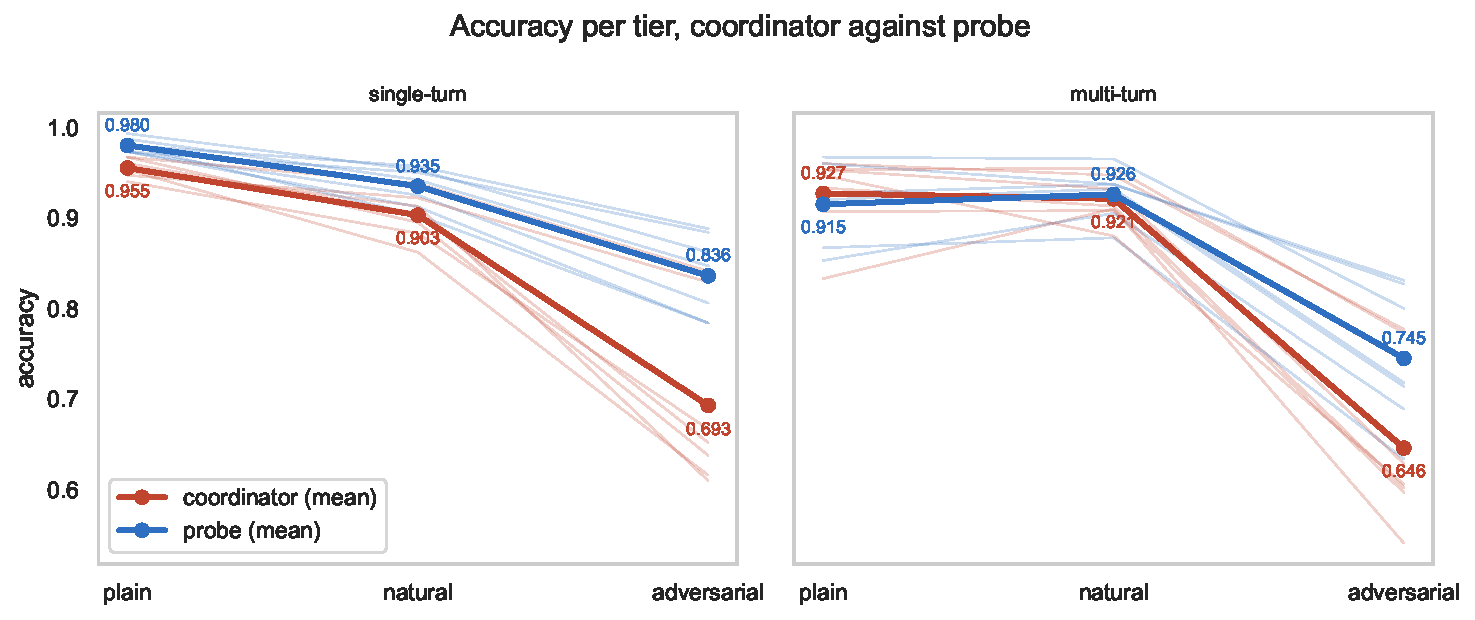
\includegraphics[width=\textwidth]{images/plots/overview/overview_tiers.pdf}
    \caption[Coordinator and probe accuracy across difficulty tiers]{Accuracy of the coordinator and of the probe on each difficulty tier, one panel per dataset. Thick lines are the mean over the seven models, thin lines are single runs. The tier drop is the fall of a line from \texttt{plain} to \texttt{adversarial}.}
    \label{fig:ch8-tiers}
\end{figure}
\FloatBarrier

The mean tier drop of the probe is 0.144 on the single-turn dataset and 0.170 on the multi-turn dataset, against 0.262 and 0.281 for the coordinator. The probe therefore loses less accuracy than the coordinator as the tier becomes harder, and the mean margin is largest on \texttt{adversarial}, 0.143 on the single-turn dataset and 0.099 on the multi-turn dataset. On the single-turn dataset, \texttt{plain} is the easiest tier and \texttt{adversarial} the hardest, for the coordinator and for the probe, in every model.

On the multi-turn dataset, the margin is positive in every model only on \texttt{adversarial}, where its mean is 0.099. On \texttt{plain} the margin is between $-$0.040 and 0.020, and the probe is more accurate than the coordinator in two of the seven models. On \texttt{natural} the margin is between $-$0.030 and 0.048, and the probe is more accurate than the coordinator in three of the seven models. The two tiers are not ordered by difficulty either. The probe is more accurate on \texttt{natural} than on \texttt{plain} in five of the seven models, and the coordinator is more accurate on \texttt{natural} than on \texttt{plain} in three of the seven models. The advantage of the probe on the multi-turn dataset therefore comes from \texttt{adversarial} alone, which holds 900 of the 1650 samples and contributes 0.054 of the mean margin of 0.055.

\FloatBarrier

\subsection{Accuracy Drop on the Multi-Turn Dataset}
\label{subsec:ch8-multi-turn}

The results of Chapter~\ref{chap:probing-results} show that the accuracy of the probe is lower on the multi-turn dataset than on the single-turn dataset for every model. Table~\ref{tab:ch8-multi-turn} reports, per model, the \emph{multi-turn drop} $\Delta_{mt}$ of the coordinator and of the probe, which is the accuracy on the multi-turn dataset minus the accuracy on the single-turn dataset. The table also reports the \emph{drop ratio}, which is the absolute multi-turn drop of the probe divided by the absolute multi-turn drop of the coordinator. The drop ratio is defined only where both multi-turn drops are negative, so it is reported for six of the seven models. The accuracies used to compute both quantities are the ones of Table~\ref{tab:ch8-overview}.

\begin{table}[htbp]
    \centering
    \small
    \begin{tabular}{@{}lccc c ccc c@{}}
        \toprule
        & \multicolumn{3}{c}{\textbf{coordinator accuracy}} & & \multicolumn{3}{c}{\textbf{probe accuracy}} & \\
        \cmidrule(lr){2-4} \cmidrule(lr){6-8}
        \textbf{Model} & \textbf{\begin{tabular}[b]{@{}c@{}}single-\\turn\end{tabular}} & \textbf{\begin{tabular}[b]{@{}c@{}}multi-\\turn\end{tabular}} & $\boldsymbol{\Delta_{mt}}$ & & \textbf{\begin{tabular}[b]{@{}c@{}}single-\\turn\end{tabular}} & \textbf{\begin{tabular}[b]{@{}c@{}}multi-\\turn\end{tabular}} & $\boldsymbol{\Delta_{mt}}$ & \textbf{\begin{tabular}[b]{@{}c@{}}drop\\ratio\end{tabular}} \\
        \midrule
        \texttt{gemma4-e2b-it}     & 0.736 & 0.702 & $-$0.034 & & 0.848 & 0.782 & $-$0.066 & 1.94 \\
        \texttt{qwen3-4b}          & 0.752 & 0.745 & $-$0.007 & & 0.864 & 0.814 & $-$0.050 & 7.14 \\
        \texttt{qwen3-8b}          & 0.772 & 0.738 & $-$0.034 & & 0.845 & 0.744 & $-$0.101 & 2.97 \\
        \texttt{gemma4-12b-it}     & 0.873 & 0.855 & $-$0.018 & & 0.916 & 0.879 & $-$0.037 & 2.06 \\
        \texttt{gemma4-26b-a4b-it} & 0.888 & 0.856 & $-$0.032 & & 0.921 & 0.878 & $-$0.043 & 1.34 \\
        \texttt{llama3.3-70b}      & 0.770 & 0.736 & $-$0.034 & & 0.894 & 0.810 & $-$0.084 & 2.47 \\
        \texttt{qwen2.5-72b}       & 0.761 & 0.768 & $+$0.007 & & 0.907 & 0.875 & $-$0.032 & N/A \\
        \bottomrule
    \end{tabular}
    \caption[Coordinator and probe accuracy across turns, with $\Delta_{mt}$]{Accuracy of the coordinator and of the probe on the single-turn and the multi-turn dataset, with the multi-turn drop $\Delta_{mt}$ and the drop ratio.}
    \label{tab:ch8-multi-turn}
\end{table}

Averaged over the seven models, the multi-turn drop is $-$0.022 for the coordinator and $-$0.059 for the probe. The multi-turn drop of the probe is larger in absolute value than the multi-turn drop of the coordinator in all seven models, including Qwen3 4B and Qwen2.5 72B, where the multi-turn drop of the coordinator accuracy is $-$0.007 and $+$0.007 but the multi-turn drop of the probe accuracy is $-$0.050 and $-$0.032. The drop ratio of Qwen2.5 72B is not defined, because its multi-turn drop of the coordinator is positive: the coordinator is more accurate on the multi-turn dataset than on the single-turn dataset, so the condition for the drop ratio, that both drops be negative, does not hold.

Figure~\ref{fig:ch8-multi-turn} draws the multi-turn drop $\Delta_{mt}$ of Table~\ref{tab:ch8-multi-turn} as one bar for the coordinator and one bar for the probe, per model.

\begin{figure}[htbp]
    \centering
    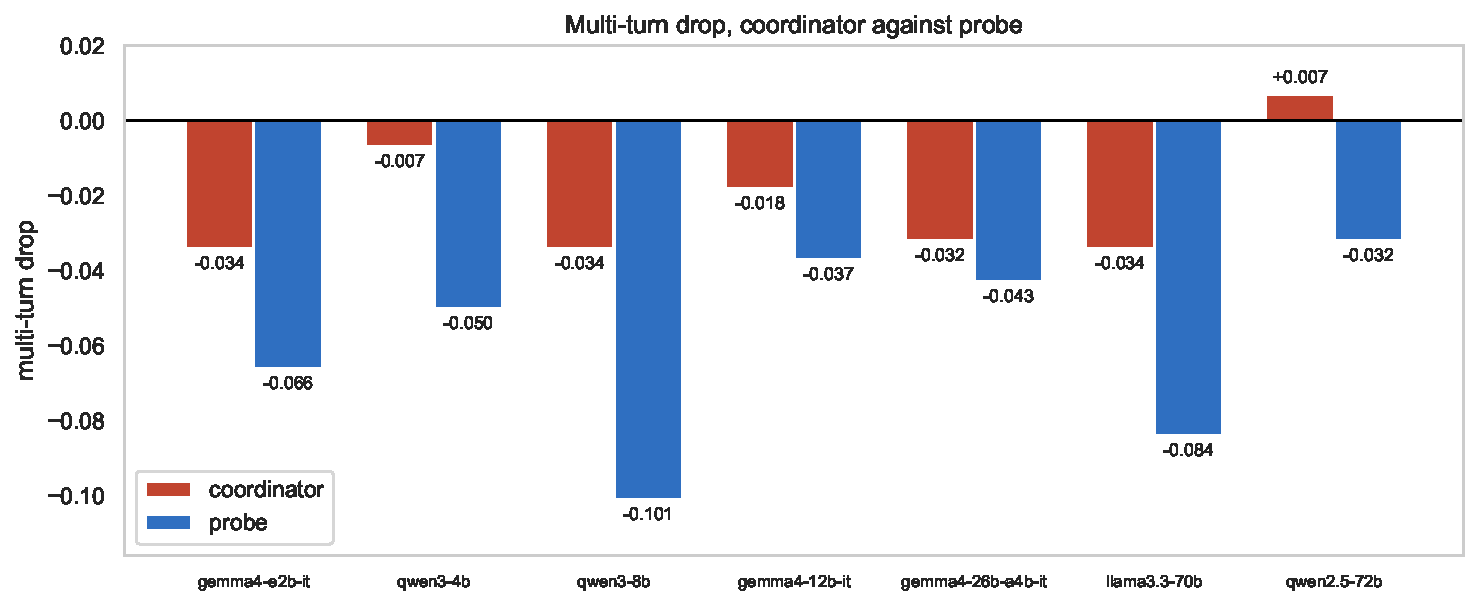
\includegraphics[width=\textwidth]{images/plots/overview/overview_multi_turn.pdf}
    \caption[Multi-turn drop $\Delta_{mt}$ of the coordinator and of the probe, per model]{Multi-turn drop $\Delta_{mt}$ of the coordinator and of the probe, per model. A bar below zero is a lower accuracy on the multi-turn dataset than on the single-turn dataset.}
    \label{fig:ch8-multi-turn}
\end{figure}

\FloatBarrier

\subsection{Answer to RQ1}
\label{subsec:ch8-rq1-answer}

\phantomsection\label{rq:ch8-rq1}
\begin{rqbox}[RQ1]
On requests where the correct sub-agent is difficult to determine from the wording alone, does a probe on the hidden states of a coordinator model recover the correct sub-agent more accurately than the coordinator's own selection?
\end{rqbox}


\noindent Yes. On both datasets and on every model of this section (GPT-OSS 20B excluded), the accuracy of the probe exceeds the accuracy of the coordinator, and the difference is significant in all the runs except Qwen3 8B on the multi-turn dataset, where the margin is 0.006. The mean margin is 0.092 on the single-turn dataset and 0.055 on the multi-turn dataset.

The advantage is largest on the \texttt{adversarial} tier, which is the difficulty tier where the correct sub-agent is the most difficult to determine from the wording of the request. On the single-turn dataset the mean margin grows from 0.025 on \texttt{plain} and 0.032 on \texttt{natural} to 0.143 on \texttt{adversarial}, and on the multi-turn dataset it grows from $-$0.012 and 0.005 to 0.099.

Every tier margin is lower in the multi-turn setting. The multi-turn drop $\Delta_{mt}$ of the probe is larger than the multi-turn drop of the coordinator in all seven models, $-$0.059 against $-$0.022 on average. A possible reason is that, in the multi-turn setting, the hidden state at the last prompt token provides a less separable representation of the sub-agents to train the probe on. Wu et al. report a similar loss of reliability while steering tool selection (adding a direction to the hidden state to change the tool the model calls): the effect becomes inconsistent once the conversation spans several turns \cite{wuToolCallingLinearly2026}.

\FloatBarrier


\section{Failure Analysis}
\label{sec:ch8-failure-analysis}

\phantomsection\label{rq:ch8-rq2-intro}
\begin{rqbox}[RQ2]
Does a probe on the coordinator's hidden states recover the correct sub-agent more accurately than classifiers trained on a fixed representation of the query text, such as raw word counts, TF-IDF weighting, or sentence embeddings?
\end{rqbox}


\noindent To answer \hyperref[rq:ch8-rq2-intro]{\textbf{RQ2}}, this section compares the probe with the three text-only classifiers on the \texttt{natural} and the \texttt{adversarial} tier. A request of the \texttt{natural} tier states a waived constraint, and the sub-agent that owns it is the decoy (Section~\ref{subsec:constraints-binding-waived}). The \texttt{adversarial} tier generates its requests in pairs: the two requests of a pair share most of their wording, and the correct sub-agent of each one is the decoy of the other (Section~\ref{subsec:difficulty-tiers}). The decoy and the pair are the cause of the lower accuracy of the text-only classifiers on these two tiers. The \texttt{plain} tier is deliberately excluded, because it introduces no difficulty and every text-only classifier scores close to ceiling accuracy on it.

The errors of the probe are first compared with the errors of each text-only classifier, to measure how much the two depend on each other. The probe, the coordinator and the text-only classifiers are then compared on how often each predicts the decoy, and on how often each predicts the same sub-agent for both requests of a pair. An advantage of the probe on these measures indicates that the binding constraint is encoded in the hidden states more accurately than in the representations of the request text that the text-only classifiers use.

\subsection{Error Dependence Across the Tiers}
\label{subsec:ch8-failure-dependence}

The errors of the probe are compared with the errors of the text-only classifiers to determine whether the hidden states encode information that the representations of the text-only classifiers do not encode. If the probe fails mostly on the same requests as a text-only classifier, its errors follow the text of the request as that classifier's errors do. If its errors are largely independent of the errors of the text-only classifiers, the hidden states are likely to encode information that these representations do not encode.

The coordinator is not included in this subsection because it is never trained on the requests of the dataset, unlike the probe and the text-only classifiers. The probe and the text-only classifiers are logistic regressions trained on the same labels and the same folds, and each receives a different input representation. A difference between their errors can therefore only come from this representation. A difference between the errors of the coordinator and the errors of a text-only classifier cannot be read the same way.

For each text-only classifier, the requests of a tier are divided into two groups: the requests where the text-only classifier is right and the requests where it is wrong. The following quantities are then computed for the probe, on each tier and against each text-only classifier:

\begin{itemize}
    \item \textbf{accuracy where the text-only classifier is right} ($a_p^{+}$): the accuracy of the probe on the requests where the text-only classifier is right;
    \item \textbf{accuracy where the text-only classifier is wrong} ($a_p^{-}$): the accuracy of the probe on the requests where the text-only classifier is wrong;
    \item \textbf{gap} ($g$): the difference $g = a_p^{-} - a_p^{+}$. A negative $g$ indicates that the probe is less accurate on the requests where the text-only classifier is wrong;
    \item \textbf{normalized kappa} ($\kappa_n$): measures how strongly the probe and the text-only classifier are right on the same requests and wrong on the same requests, on a scale from 0 for independent errors to 1 for the strongest agreement that the accuracies of the two allow.
\end{itemize}

The normalized kappa is derived from Cohen's kappa. For the probe and a text-only classifier, Cohen's kappa is computed as
\[
    \kappa = \frac{p_o - p_e}{1 - p_e},
\]
where:

\begin{itemize}
    \item $p_o$ is the fraction of requests on which the probe and the text-only classifier are both right or both wrong;
    \item $p_e$ is the value of $p_o$ expected from the accuracy of the probe and the accuracy of the text-only classifier if their errors were independent.
\end{itemize}

The highest value that $\kappa$ can reach depends on the accuracy $a_p$ of the probe and the accuracy $a_b$ of the text-only classifier. When the two accuracies differ, one of the two is right and the other is wrong on at least a fraction $|a_p - a_b|$ of the requests. Therefore $p_o$ is at most $1 - |a_p - a_b|$, and $\kappa$ is at most
\[
    \kappa_{\max} = \frac{1 - |a_p - a_b| - p_e}{1 - p_e}.
\]
The accuracies of the probe and of the text-only classifiers differ across text-only classifiers and tiers, so $\kappa_{\max}$ differs too, and the same value of $\kappa$ can indicate a weak agreement in one row of the comparison and a strong agreement in another. The normalized kappa removes this effect by dividing $\kappa$ by its highest reachable value:
\[
    \kappa_n = \frac{\kappa}{\kappa_{\max}}.
\]

If the errors of the probe do not depend on the errors of the text-only classifier, $g$ and $\kappa_n$ are close to 0 in absolute value. If the probe and the text-only classifier are right on the same requests and wrong on the same requests, $g$ is large and negative and $\kappa_n$ is close to 1. Table~\ref{tab:ch8-dependence} reports $a_p^{+}$, $a_p^{-}$, $g$ and $\kappa_n$ on the \texttt{natural} and \texttt{adversarial} tiers, and Figure~\ref{fig:ch8-dependence} plots $a_p^{+}$, $a_p^{-}$ and $g$.

In every row of Table~\ref{tab:ch8-dependence}, $a_p^{-}$ is lower than $a_p^{+}$, with $g$ between $-$0.028 and $-$0.179. Some of the requests on which the wording misleads the text-only classifiers therefore also mislead the probe. $\kappa_n$ between the probe and a text-only classifier is between 0.151 and 0.424. The absolute value of $g$ is larger on \texttt{adversarial} than on \texttt{natural} for every combination of dataset and text-only classifier. This shows that the difficulty of \texttt{adversarial} affects the probe more on the requests where a text-only classifier is wrong. Against the bag-of-words classifier, $\kappa_n$ is lower on \texttt{adversarial} than on \texttt{natural} on both datasets. Against the TF-IDF classifier, it is higher on the single-turn dataset and lower on the multi-turn dataset. Against the embedding classifier, it is higher on both datasets.

\begin{table}[H]
    \centering
    \small
    \begin{tabular}{@{}llcccc c cccc@{}}
        \toprule
        & & \multicolumn{4}{c}{\textbf{Single-turn}} & & \multicolumn{4}{c}{\textbf{Multi-turn}} \\
        \cmidrule(lr){3-6} \cmidrule(lr){8-11}
        \textbf{Tier} & \textbf{Classifier} & $\boldsymbol{a_p^{+}}$ & $\boldsymbol{a_p^{-}}$ & $\boldsymbol{g}$ & $\boldsymbol{\kappa_n}$ & & $\boldsymbol{a_p^{+}}$ & $\boldsymbol{a_p^{-}}$ & $\boldsymbol{g}$ & $\boldsymbol{\kappa_n}$ \\
        \midrule
        \texttt{natural}     & Bag-of-words & 0.958 & 0.878 & $-$0.080 & 0.356 & & \worst{0.944} & 0.891 & $-$0.053 & \worst{0.243} \\
                             & TF-IDF       & \best{0.959} & \worst{0.868} & \worst{$-$0.091} & \best{0.367} & & \best{0.950} & \worst{0.876} & \worst{$-$0.074} & \best{0.366} \\
                             & Embedding    & \worst{0.944} & \best{0.916} & \best{$-$0.028} & \worst{0.151} & & \worst{0.944} & \best{0.900} & \best{$-$0.044} & 0.268 \\
        \midrule
        \texttt{adversarial} & Bag-of-words & 0.888 & 0.749 & $-$0.139 & \worst{0.317} & & \worst{0.795} & 0.670 & \best{$-$0.125} & \worst{0.204} \\
                             & TF-IDF       & \best{0.905} & \worst{0.748} & \worst{$-$0.157} & \best{0.424} & & \best{0.833} & \worst{0.654} & \worst{$-$0.179} & \best{0.362} \\
                             & Embedding    & \worst{0.886} & \best{0.791} & \best{$-$0.095} & 0.321 & & 0.820 & \best{0.692} & $-$0.128 & 0.298 \\
        \bottomrule
    \end{tabular}
    \caption[Probe accuracy by classifier correctness, gap, and normalized kappa]{Accuracy of the probe on the requests where each text-only classifier is right ($a_p^{+}$) and on the requests where it is wrong ($a_p^{-}$), gap $g = a_p^{-} - a_p^{+}$, and normalized kappa $\kappa_n$ between the probe and the text-only classifier. Each value is the mean of the seven runs on the same dataset. In each tier and column, the highest value is in bold and the lowest is underlined.}
    \label{tab:ch8-dependence}
\end{table}

\begin{figure}[htbp]
    \centering
    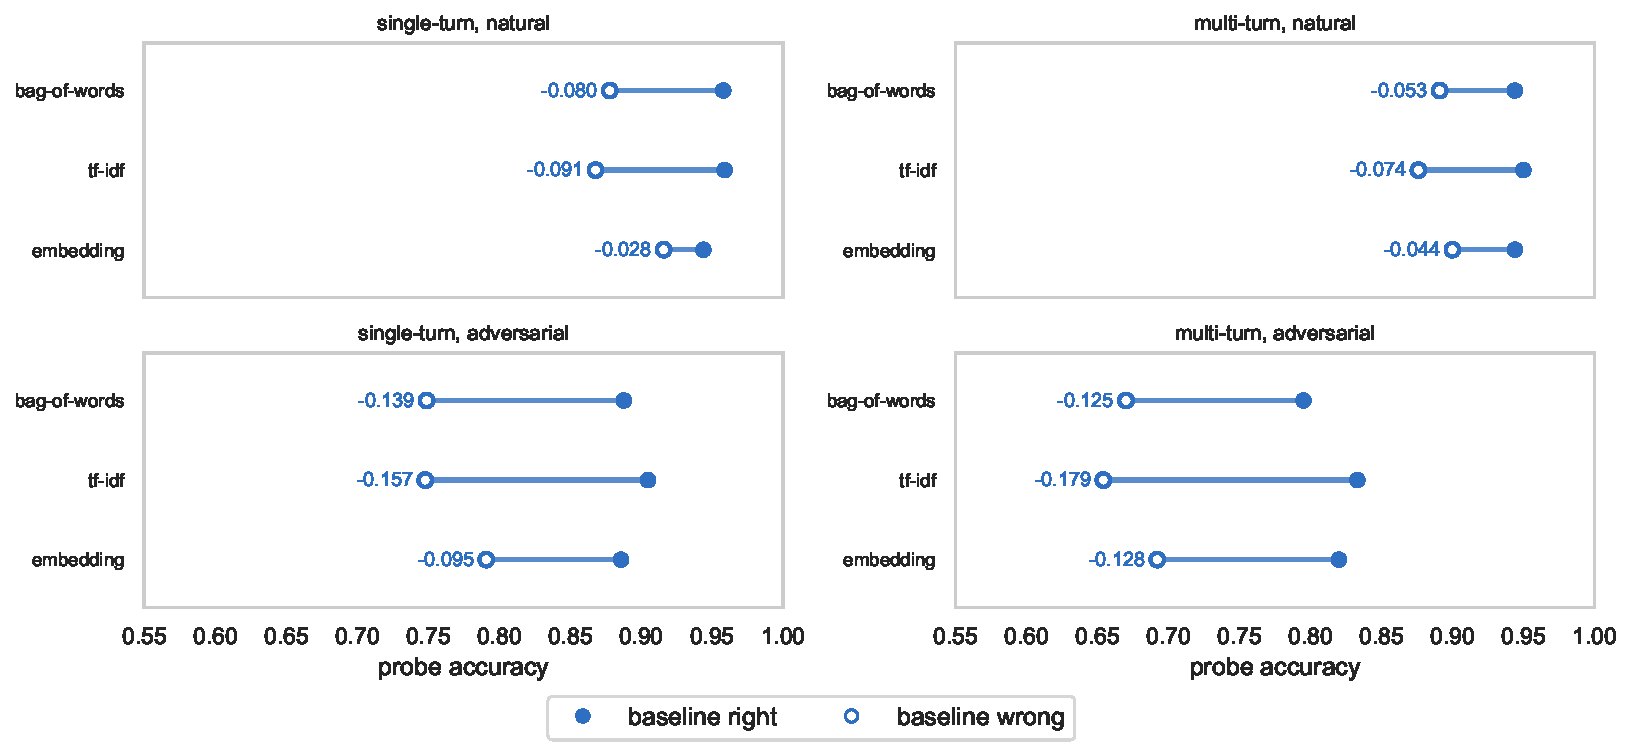
\includegraphics[width=\textwidth]{images/plots/overview/overview_dependence.pdf}
    \caption[Probe accuracy where each text-only classifier is right and where it is wrong]{Accuracy of the probe where each text-only classifier is right ($a_p^{+}$, filled end) and where it is wrong ($a_p^{-}$, hollow end), one panel per dataset and tier. The number at the hollow end is the gap $g$. Each value is the mean of the seven runs on the same dataset.}
    \label{fig:ch8-dependence}
\end{figure}

\FloatBarrier

\subsection{Adversarial Pairs}
\label{subsec:ch8-failure-pairs}

As described in Section~\ref{subsec:difficulty-tiers}, the \texttt{adversarial} tier of each dataset consists of 900 samples generated in 450 pairs. The two requests of a pair share most of their wording and differ only in the clause that names the constraint that is binding. Both requests state the same two constraints, and the constraint that is binding in one request is waived in the other, so the correct sub-agent of each request is the decoy of the other. The pairs are used to observe whether a classifier tells the two requests of a pair apart or predicts the same sub-agent for both, where a \emph{classifier} is any of the probe, the coordinator and the three text-only classifiers. Two quantities are computed for each classifier:

\begin{itemize}
    \item \textbf{both, one or neither right}: the share of pairs in which the classifier classifies both requests correctly, one of the two, or neither;
    \item \textbf{collapsed pairs}: the share of pairs in which the classifier predicts the same sub-agent for both requests. In a collapsed pair, at most one of the two requests is classified correctly.
\end{itemize}

Figure~\ref{fig:ch8-pairs} reports both quantities and shows that the probe is the only classifier that classifies both requests correctly in most pairs, on both datasets. The coordinator and the text-only classifiers classify only one of the two requests correctly in most pairs.

\begin{figure}[htbp]
    \centering
    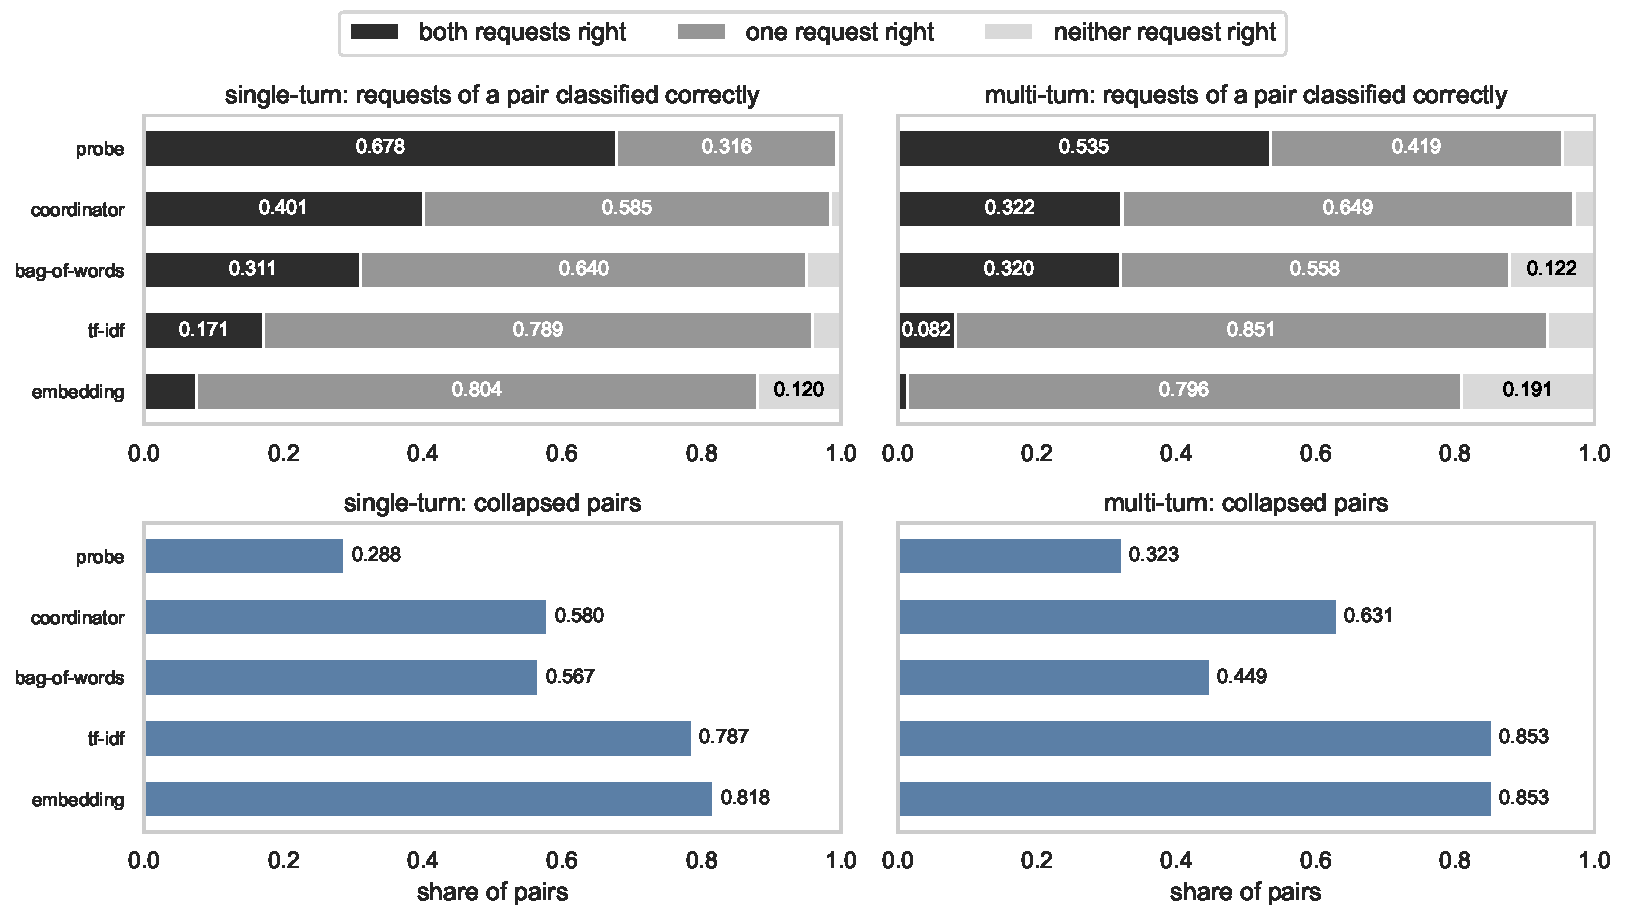
\includegraphics[width=\textwidth]{images/plots/overview/overview_pairs.pdf}
    \caption[Adversarial pair correctness and collapsed pairs per classifier]{Top: share of the 450 \texttt{adversarial} pairs in which each classifier classifies both, one or neither of the two requests correctly. Bottom: share of collapsed pairs. Single-turn dataset on the left, multi-turn dataset on the right. The probe and the coordinator values are the mean of the seven runs on the same dataset. The text-only classifiers do not depend on the model.}
    \label{fig:ch8-pairs}
\end{figure}

The probe collapses fewer pairs than the coordinator on both datasets, with a mean share of collapsed pairs of 0.288 and 0.323 against 0.580 and 0.631. The coordinator collapses fewer pairs than the TF-IDF and embedding classifiers, but more than the bag-of-words classifier, which has a share of collapsed pairs of 0.567 and 0.449. The probe also has the highest share of pairs with both requests right on both datasets, with a mean of 0.678 and 0.535 against 0.401 and 0.322 for the coordinator.

\FloatBarrier

\subsection{Decoy Predictions}
\label{subsec:ch8-failure-decoy}

On \texttt{natural} and \texttt{adversarial}, every request states a waived constraint, and the sub-agent that owns it is the decoy (Section~\ref{subsec:constraints-binding-waived}). The decoy predictions are used to observe how often each classifier is misled by the waived constraint, and whether the probe is misled less often than the coordinator and the text-only classifiers. The \emph{decoy rate} of a classifier is defined as the share of the samples of a tier on which the classifier predicts the decoy. Figure~\ref{fig:ch8-decoy} reports the decoy rate of every classifier.

\begin{figure}[htbp]
    \centering
    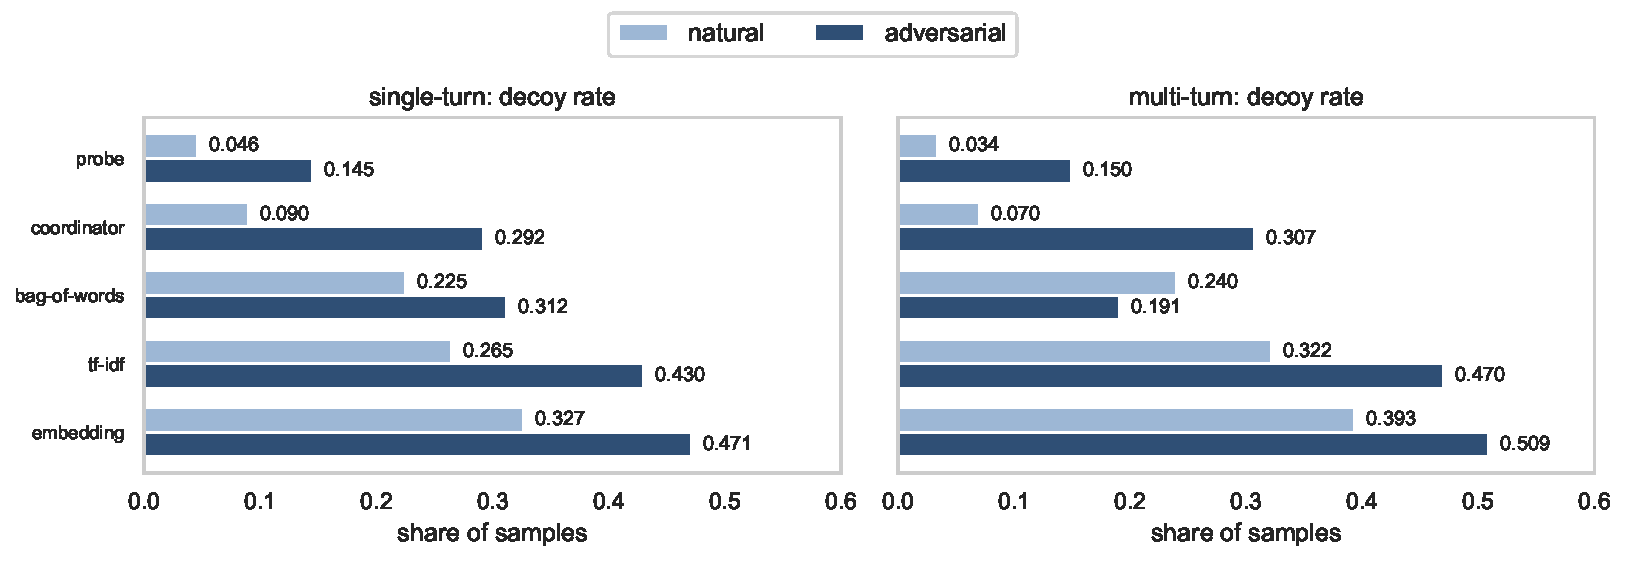
\includegraphics[width=\textwidth]{images/plots/overview/overview_decoy.pdf}
    \caption[Decoy rate by tier, single-turn and multi-turn datasets]{Decoy rate: share of the samples of each tier on which each classifier predicts the decoy, single-turn dataset on the left and multi-turn dataset on the right. The probe and the coordinator values are the mean of the seven runs on the same dataset. The text-only classifiers do not depend on the model.}
    \label{fig:ch8-decoy}
\end{figure}

The probe has the lowest mean decoy rate on both tiers and both datasets. The coordinator has the second lowest, except on the multi-turn \texttt{adversarial} tier, where the bag-of-words classifier has the second lowest.

The probe improves on the coordinator in the three measures of this section: on both datasets it has a lower mean share of collapsed pairs, a higher mean share of pairs with both requests right, and a lower mean decoy rate on both tiers. The correct sub-agent is therefore encoded in the hidden states of the coordinator, but the coordinator does not select it as accurately as the probe. This may come from the training of the probe, which learns to read the sub-agent from the hidden states on labeled samples of the dataset, while the coordinator chooses according to the routing policy stated in its prompt.

\subsection{Answer to RQ2}
\label{subsec:ch8-rq2-answer}

\phantomsection\label{rq:ch8-rq2}
\begin{rqbox}[RQ2]
Does a probe on the coordinator's hidden states recover the correct sub-agent more accurately than classifiers trained on a fixed representation of the query text, such as raw word counts, TF-IDF weighting, or sentence embeddings?
\end{rqbox}


\noindent Yes. Section~\ref{sec:ch7-observations} reports that the probe is more accurate than all three text-only classifiers on the \texttt{natural} and the \texttt{adversarial} tier of both datasets.

On the \texttt{adversarial} pairs, the probe has the lowest mean share of collapsed pairs and the highest mean share of pairs with both requests right on both datasets, and it has the lowest mean decoy rate on both tiers and both datasets. The binding constraint stated in a request can therefore be read more accurately from the hidden state at the last prompt token than from the representations of the request text that the text-only classifiers use.

The advantage is partial, because the errors of the probe partly follow the errors of the text-only classifiers: $a_p^{-}$ is lower than $a_p^{+}$ in every comparison of Table~\ref{tab:ch8-dependence}, with $\kappa_n$ between 0.151 and 0.424.

\FloatBarrier


\section{Relative Depth of the Optimal Layer}
\label{sec:ch8-depth}

\phantomsection\label{rq:ch8-rq3-intro}
\begin{rqbox}[RQ3]
Does the optimal probe layer fall at a consistent relative depth across different LLMs?
\end{rqbox}


\noindent To answer \hyperref[rq:ch8-rq3-intro]{\textbf{RQ3}}, this section measures where the optimal layer of each run falls in the stack of layers of its model (Section~\ref{subsec:block}), expressed as a fraction of the number of layers, called the \emph{relative depth}. Section~\ref{sec:ch7-results} reports the optimal layer of each run, the layer at which the probe reaches its highest accuracy. That layer index does not compare directly across models, because the layer count in the pool ranges from 30 to 80, so a specific layer does not mark the same depth in every model. A relative depth that is similar across the models indicates that the routing signal concentrates at the same relative depth in every model.

\subsection{Relative Depth of the Optimal Layer per Run}
\label{subsec:ch8-depth-values}

Each optimal layer is divided by the last layer index, which places it in $[0, 1]$ and gives its relative depth. This rescaling makes the positions comparable across models. Figure~\ref{fig:ch8-depth} plots the relative depth of the optimal layer for the fourteen runs.

\begin{figure}[htbp]
    \centering
    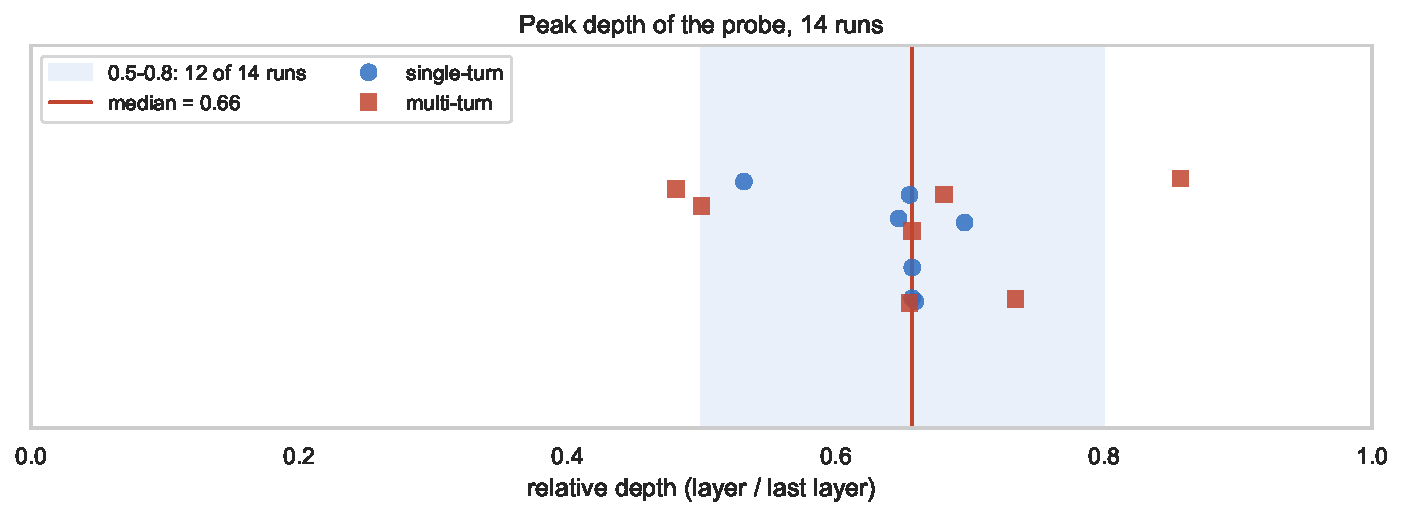
\includegraphics[width=\textwidth]{images/plots/overview/overview_depth.pdf}
    \caption[Relative depth of the probe's optimal layer]{Relative depth of the probe's optimal layer, fourteen runs.}
    \label{fig:ch8-depth}
\end{figure}

The median relative depth is 0.66, with quartiles at 0.65 and 0.68. Twelve of the fourteen runs fall between 0.5 and 0.8. The two remaining runs fall outside that range: Llama 3.3 70B multi-turn at 0.48, 0.02 below the lower bound, and Qwen3 8B multi-turn at 0.86, 0.06 above the upper bound. The single-turn and the multi-turn runs give the same median, so the number of turns does not move the relative depth of the optimal layer, but the two groups differ in spread: the standard deviation of the relative depth is 0.05 for the single-turn runs and 0.13 for the multi-turn runs. Section~\ref{subsec:ch8-multi-turn} relates the larger multi-turn drop in probe accuracy to a less separable representation of the sub-agents in the multi-turn hidden states, and the same reduced separability could also explain why the multi-turn relative depth is less consistent across models.

Ratnakar et al. note that deeper layers dominate in typical probing results, but their own LatentGate results differ: the optimal layer falls at a relative depth of 0.25 to 0.50 \cite{ratnakarLatentGateLowLatencySemantic2026}. They give as a likely reason that their agent-routing task requires broad topic discrimination rather than fine-grained linguistic analysis. The median relative depth of 0.66 here is larger, so the optimal layer falls in the second half of the layer stack. The routing task in this work requires deciding which of several constraints binds on a shared scenario, a finer-grained judgment than topic-level agent selection. Following the explanation of Ratnakar et al., this finer-grained judgment may be the reason why the optimal layer falls deeper than in LatentGate.

\subsection{Answer to RQ3}
\label{subsec:ch8-rq3-answer}

\phantomsection\label{rq:ch8-rq3}
\begin{rqbox}[RQ3]
Does the optimal probe layer fall at a consistent relative depth across different LLMs?
\end{rqbox}


\noindent Yes. The relative depth of the optimal layer lies between 0.5 and 0.8 in twelve of the fourteen runs, with a median of 0.66 that is the same on the single-turn and on the multi-turn dataset.

The consistency is lower in the multi-turn setting. Both runs outside the 0.5 to 0.8 band are multi-turn, Llama 3.3 70B at 0.48 and Qwen3 8B at 0.86, and the standard deviation of the relative depth is 0.13 on the multi-turn dataset against 0.05 on the single-turn dataset.

The claim that the optimal layer occurs at a consistent relative depth is limited to the pool of models analyzed in this work, which is too small to provide a valid generalization.

\FloatBarrier


\section{The Probe as an Evaluation Flag}
\label{sec:ch8-error-flag}

\phantomsection\label{rq:ch8-rq4-intro}
\begin{rqbox}[RQ4]
Can the disagreement between the probe and the coordinator be used as a runtime flag for likely misrouting?
\end{rqbox}


\noindent To answer \hyperref[rq:ch8-rq4-intro]{\textbf{RQ4}}, the probe is measured as a flag for a likely misroute. Section~\ref{sec:ch8-overview} shows that the probe is more accurate than the coordinator on the whole dataset, in all the runs. When the probe and the coordinator predict a different sub-agent for the same request, at most one of them is right, and the coordinator is the more likely one to be wrong, because it is the less accurate of the two. The \emph{disagreement flag} is raised on a sample when the out-of-fold prediction of the probe differs from the sub-agent predicted by the coordinator. The flag is measured against the error rate of the coordinator, to determine whether it marks the misroutes more often than the base rate and how many correct decisions it marks by mistake.

\subsection{Metrics}
\label{subsec:ch8-error-flag-metrics}

Four metrics are used to measure the quality of the disagreement flag. Each metric treats an error of the coordinator as the positive class and a raised flag as a positive prediction:

\begin{itemize}
    \item \textbf{precision}: the share of the flagged samples where the coordinator is wrong,
    \[
        P(\text{coordinator wrong} \mid \text{flagged})
    \]
    \item \textbf{recall}: the share of the coordinator's errors that are flagged,
    \[
        P(\text{flagged} \mid \text{coordinator wrong})
    \]
    \item \textbf{F1-score}: the harmonic mean of precision and recall, a single value for how well the flag covers the coordinator's errors,
    \[
        2 \cdot \frac{\text{precision} \cdot \text{recall}}{\text{precision} + \text{recall}}
    \]
    \item \textbf{false positive rate} (FPR): the share of the coordinator's correct decisions that are flagged, the same metric that Section~\ref{subsec:ch7-metrics} uses for the ROC curve,
    \[
        P(\text{flagged} \mid \text{coordinator right})
    \]
\end{itemize}

The \emph{base error rate} is the share of the samples of a run where the coordinator predicts the wrong sub-agent, and it varies from 0.112 to 0.298 across the runs. A low base error rate leaves few errors for the flag to hit, which lowers precision and the F1-score. Precision and the F1-score must therefore be read against the base error rate of their own run, reported next to them. The F1-score measures the quality of the flag on one run. A model with a high base error rate gives the flag more errors to find, so it can reach a higher F1-score while its coordinator routes less accurately.

The F1-score is computed from precision and recall only, so it does not count the correct decisions of the coordinator that the flag leaves unmarked. The false positive rate measures the share of the correct decisions that are flagged by the probe.

\subsection{Results}
\label{subsec:ch8-error-flag-results}

Table~\ref{tab:ch8-error-flag} reports the four metrics of each run, together with the base error rate of the coordinator and the margin $\Delta$ of Table~\ref{tab:ch8-overview}.

The precision of the flag (the share of the flagged samples where the coordinator is wrong) is between 0.598 and 0.826. In each of the fourteen runs it exceeds the base error rate of the coordinator in that same run, which is between 0.112 and 0.298. The recall (the share of the errors of the coordinator that are flagged) is between 0.540 and 0.797. The false positive rate is between 0.028 and 0.160, and below 0.100 in twelve of the runs. The F1-score, which combines precision and recall, is between 0.601 and 0.811.

The flag is less reliable on the multi-turn dataset. Its false positive rate rises for six of the seven models, by between 0.015 and 0.068, and is unchanged for Qwen2.5 72B. The probe loses more accuracy than the coordinator in the multi-turn setting (Section~\ref{subsec:ch8-multi-turn}), and a probe with lower accuracy raises the flag on more of the correct decisions of the coordinator.

\begin{table}[H]
    \centering
    \small
    \begin{tabular}{@{}lcccccc@{}}
        \toprule
        \textbf{Model} & \textbf{Precision} & \textbf{Recall} & \textbf{F1-score} & \textbf{Base error} & \textbf{FPR} & $\boldsymbol{\Delta}$ \\
        \midrule
        \multicolumn{7}{@{}l}{\textit{Single-turn}} \\
        \midrule
        \texttt{gemma4-e2b-it}     & 0.738 & 0.700 & 0.718 & 0.264 & 0.089 & 0.112 \\
        \texttt{qwen3-4b}          & 0.756 & 0.717 & 0.736 & 0.248 & 0.077 & 0.112 \\
        \texttt{qwen3-8b}          & 0.683 & 0.670 & 0.677 & 0.228 & \worst{0.092} & 0.073 \\
        \texttt{gemma4-12b-it}     & 0.741 & 0.560 & \worst{0.638} & 0.127 & \best{0.028} & 0.043 \\
        \texttt{gemma4-26b-a4b-it} & 0.681 & 0.600 & \worst{0.638} & 0.112 & 0.035 & 0.033 \\
        \texttt{llama3.3-70b}      & 0.779 & 0.763 & 0.771 & 0.230 & 0.065 & 0.124 \\
        \texttt{qwen2.5-72b}       & 0.826 & 0.797 & \best{0.811} & 0.239 & 0.053 & 0.146 \\
        \midrule
        \multicolumn{7}{@{}l}{\textit{Multi-turn}} \\
        \midrule
        \texttt{gemma4-e2b-it}     & 0.712 & 0.778 & 0.744 & 0.298 & 0.134 & 0.080 \\
        \texttt{qwen3-4b}          & 0.703 & 0.688 & 0.696 & 0.255 & 0.099 & 0.069 \\
        \texttt{qwen3-8b}          & 0.598 & 0.671 & 0.632 & 0.262 & \worst{0.160} & 0.006 \\
        \texttt{gemma4-12b-it}     & 0.679 & 0.540 & \worst{0.601} & 0.145 & \best{0.043} & 0.024 \\
        \texttt{gemma4-26b-a4b-it} & 0.673 & 0.639 & 0.655 & 0.144 & 0.052 & 0.022 \\
        \texttt{llama3.3-70b}      & 0.736 & 0.653 & 0.692 & 0.264 & 0.084 & 0.074 \\
        \texttt{qwen2.5-72b}       & 0.805 & 0.725 & \best{0.763} & 0.232 & 0.053 & 0.107 \\
        \bottomrule
    \end{tabular}
    \caption[Probe read as a flag on the coordinator's decision]{The probe read as a flag on the coordinator's decision: precision, recall, the F1-score, the coordinator's base error rate, the false positive rate (FPR), and the margin $\Delta$ of Table~\ref{tab:ch8-overview}. In each dataset, the best F1-score and FPR are in bold and the worst are underlined.}
    \label{tab:ch8-error-flag}
\end{table}

\FloatBarrier

\subsection{Answer to RQ4}
\label{subsec:ch8-rq4-answer}

\phantomsection\label{rq:ch8-rq4}
\begin{rqbox}[RQ4]
Can the disagreement between the probe and the coordinator be used as a runtime flag for likely misrouting?
\end{rqbox}


\noindent Yes. For every model, on both datasets, the precision of the flag is between 0.598 and 0.826 and above the base error rate of that model, which is between 0.112 and 0.298. The recall is between 0.540 and 0.797, and the false positive rate is between 0.028 and 0.160, below 0.100 in twelve of the fourteen runs.

The flag is less reliable in the multi-turn setting, where its false positive rate rises for six of the seven models, by between 0.015 and 0.068.

\FloatBarrier


\flushbottom
